
%(BEGIN_QUESTION)
% Copyright 2015, Tony R. Kuphaldt, released under the Creative Commons Attribution License (v 1.0)
% This means you may do almost anything with this work of mine, so long as you give me proper credit

Calculate all voltages and all currents in this transformer circuit, assuming the 3.3 k$\Omega$ resistor drops 13 volts:

$$\includegraphics[width=15.5cm]{i01273x01.eps}$$

\begin{itemize}
\item{} $V_{source}$ = 
\item{} $V_{primary}$ = 
\item{} $V_{secondary}$ = 
\item{} $I_{source}$ =  
\item{} $I_{primary}$ = 
\item{} $I_{secondary}$ = 
\end{itemize}

\underbar{file i01273}
%(END_QUESTION)





%(BEGIN_ANSWER)

\begin{itemize}
\item{} $V_{source}$ = 5.32 V
\item{} $V_{primary}$ = 4.763 V
\item{} $V_{secondary}$ = 14.97 V
\item{} $I_{source}$ = 12.38 mA
\item{} $I_{primary}$ = 12.38 mA
\item{} $I_{secondary}$ = 3.939 mA
\end{itemize}
 
%(END_ANSWER)





%(BEGIN_NOTES)


%INDEX% Electronics review: transformer ratios

%(END_NOTES)


